\documentclass[a4paper,10pt]{exam}

\usepackage[utf8]{inputenc}
\usepackage[cyr]{aeguill}
\usepackage[francais]{babel}
\usepackage{fullpage}
\usepackage{amsmath}
\usepackage{array}
\usepackage{tikz}
\input kvmacros
\usetikzlibrary{arrows,shapes,trees,patterns,fit,backgrounds,%
decorations.pathreplacing,chains,calc,decorations.pathmorphing,matrix,circuits.logic.CDH,automata}

\ifthenelse{\equal{\detokenize{correction}}{\jobname}}
{\printanswers}
{\noprintanswers}

\title{Architecture des ordinateurs - TD 10}

\author{}
\date{}

\begin{document}
\maketitle

\section{Échauffement: Quine McCluskey}
$$ f(a,b,c,d) = \sum m(2,3,7,9,11,13) + \sum d(1,10,15) $$
\begin{itemize}
  \item Réduire la fonction $f$ par la méthode de Quine McCluskey.
\end{itemize}

\section{Additionneur à Retenue anticipée}

\subsection{Rappels: Additionneur Série}

Le circuit d'un additionneur complet est donné ci-dessous:

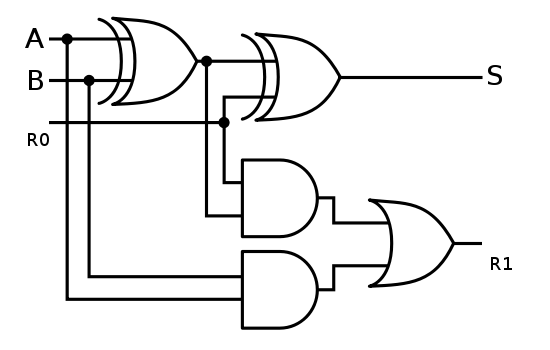
\includegraphics[width=3cm]{TD10-Fadd}

\begin{enumerate}
  \item Rappeler le circuit d'un additionneur 4 bits série:
    \begin{solution}
    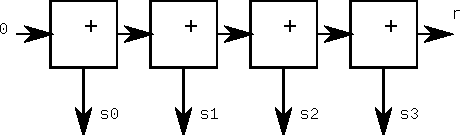
\includegraphics{TD10-Sadd4}
    \end{solution}


    Le chemin critique dans un circuit électronique représente le chemin
    le plus long entre les entrées et les sorties. On l'exprimera ici en
    nombre de portes. Le chemin critique permet de calculer le temps nécessaire
    pour obtenir un résultat dans un circuit combinatoire.

  \item Quelle est la longueur du chemin critique dans ce circuit (en nombre de
    portes traversées ) ?
  \item Quelle est la longueur du chemin critique pour un additionneur $n$ bits
    série ?
\end{enumerate}

\subsection{Additionneur à retenue anticipée}
Les additionneurs à retenue anticipée permettent d'accélérer le temps de
propagation dans un additionneur. Pour cela ils réduisent le nombre de portes
nécessaires pour propager la retenue à travers le circuit.  On va implémenter un
additionneur à retenue anticipée (Carry Lookahead Adder).

\begin{enumerate}
\item Lorsqu'un additionneur complet génère une retenue, deux scénarios sont
  possibles: l'additionneur génère une retenue lors de la somme ou
  l'additionneur propage la retenue de l'additionneur précédent.  Modifiez le
  circuit de l'additionneur complet de manière à rajouter deux signaux sortants:
  \begin{itemize}
    \item $P$, vrai lorsque l'additionneur propage la retenue précédente.
    \item $G$, vrai lorsque l'additionneur génère une retenue.
  \end{itemize}
  Les signaux $P$ et $G$ doivent être calculés uniquement à partir de $A$ et de
  $B$.
\begin{solution}
  \begin{enumerate}
  \item $P = A + B$
  \item $G = A.B$
  \end{enumerate}
\end{solution}

Nous donnons ci-dessous le schéma général d'un additionneur
à retenue anticipée. Au lieu de propager la retenue à travers
l'ensemble des additionneurs complets, l'unité CLA va directement
calculer les retenues $R_0$,$R_1$,$R_2$ et $R_3$ de manière à réduire
la taille du chemin critique.

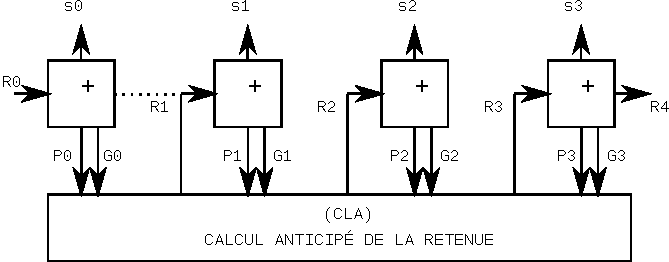
\includegraphics{TD10-CLA1}
\item Exprimez $R_1$ en fonction de $P_0$,$G_0$ et $R_0$?
\begin{solution}
  $$ R_1 = G_0 + P_0.C_0 $$
\end{solution}

\item Exprimez $R_2$ en fonction de $P_1$, $G_1$, $P_0$, $G_0$ et $R_0$.
\begin{solution}
  $$ R_2 = G_1 + P_1.C_1 = G_1 + P_1.(G_0 + P_0.C_0) = G_1 + P_1.G_0 + P_0.P_1.C_0$$
\end{solution}

\item Montrez par récurrence que
  $$R_i = G_i + \sum^{i-1}_{j=0}{(G_j.\prod^i_{k=j+1}{P_k})} + C_0.\prod^i_{j=0}{P_j}$$

\begin{solution}
  Cas de base $i=1$: $R_1 = G_0 + C_0.P_0$ vérifie l'équation.

  Récurrence, supposons l'hypothèse vraie pour $i$:
  $$R_i = G_i + \sum^{i-1}_{j=0}{(G_j.\prod^i_{k=j+1}{P_k})} +
  C_0.\prod^i_{j=0}{P_j}$$

  $$R_{i+1} = G_{i+1} + P_{i+1}.C_{i}$$

  $$R_{i+1} = G_{i+1} + P_{i+1}.(G_i + \sum^{i-1}_{j=0}{(G_j.\prod^i_{k=j+1}{P_k})} +
  C_0.\prod^i_{j=0}{P_j})$$

  $$ R_{i+1} = G_{i+1} + \sum^{i-1}_{j=0}{(G_j.\prod^i_{k=j+1}{P_k})} +
  C_0.\prod^{i+1}_{j=0}{P_j})$$
\end{solution}

\item En utilisant les équations précédentes, proposez un circuit pour le CLA.
\item Quelle est la longueur du chemin critique pour l'additionneur à retenue
  anticipée ?
\begin{solution}

\end{solution}

\item Bonus : Peut-on utiliser la même méthode pour implémenter un additionneur
  16 bits avec CLA ? 64 bits ? Quels sont les inconvénients ? Comment feriez
  vous pour implémenter un additionneur 16 bits avec CLA.
\end{enumerate}

\end{document}
